\documentclass[11pt]{article}
\usepackage[a4paper,margin=1.6cm]{geometry}
\usepackage{booktabs,longtable,graphicx,array}
\newcolumntype{P}[1]{>{\raggedright\arraybackslash}p{#1}}
\makeatletter
\setlength{\@fptop}{0pt}
\makeatother
\begin{document}
\section*{Supplementary Material}
\subsection*{Table S1. Parameter design space, engineering constraints, and selected levels}
The selected levels were engineering operating points chosen after qualitative screening rather than optimized values or formal physical safety limits. Their intended directional effects describe the controller or API behavior on this platform and in this task; they should not be interpreted as independently identified material properties or fingertip-force measurements.
\small
\renewcommand{\arraystretch}{1.16}
\begin{longtable}{P{0.16\textwidth}P{0.29\textwidth}P{0.27\textwidth}P{0.14\textwidth}}
\toprule
Parameter & Low-to-high operational effect & Engineering constraint & Selected levels \\
\midrule
Slave impedance: $K_t$ & Lower $K_t$ $\rightarrow$ greater translational compliance and lower impact; higher $K_t$ $\rightarrow$ greater positional resistance. & No sustained oscillation during qualitative screening. & 50 / 150 / 200 N/m \\
Slave impedance: $K_r$ & Lower $K_r$ $\rightarrow$ greater rotational compliance; higher $K_r$ $\rightarrow$ greater orientation retention against rotational disturbance. & No sustained oscillation during qualitative screening. & 5 / 10 / 13 N\,m/rad \\
Slave impedance: $\zeta$ & Increasing $\zeta$ $\rightarrow$ increasing normalized controller damping action for fixed $\mathbf{K}$; it is not a physical critical-damping ratio. & Avoid sustained oscillation and excessive sluggishness. & 0.8 / 1.0 / 1.2 \\
Master haptic: $K_f$ & Lower $K_f$ $\rightarrow$ weaker rendered external-force cue; higher $K_f$ $\rightarrow$ stronger cue. & Acceptable Omega.7 response. & 0.2 / 0.5 / 0.7 \\
Master haptic: $d$ & Lower $d$ $\rightarrow$ greater sensitivity to small forces; higher $d$ $\rightarrow$ greater suppression of small signals. & Limit master-side haptic jitter and noise. & 0.3 / 0.4 / 0.5 N \\
Gripper: $v_g$ & Lower $v_g$ $\rightarrow$ slower, lower-impact closing; higher $v_g$ $\rightarrow$ faster grasp establishment. & Franka Hand execution range. & 0.02 / 0.05 / 0.10 m/s \\
Gripper: $F_g$ & Lower requested $F_g$ $\rightarrow$ gentler grasping; higher $F_g$ $\rightarrow$ greater requested grasp force. & Franka Hand force setting. & 8 / 15 / 20 N \\
\bottomrule
\end{longtable}
\normalsize

\subsection*{Table S2. Preassigned chronological mode sequences}
\begin{tabular}{lll}
\toprule
Operator ID & Group & Mode sequence \\
\midrule
P01 & 1 & A $\rightarrow$ D $\rightarrow$ C $\rightarrow$ B $\rightarrow$ E \\
P01 & 2 & B $\rightarrow$ E $\rightarrow$ D $\rightarrow$ C $\rightarrow$ A \\
P01 & 3 & C $\rightarrow$ A $\rightarrow$ E $\rightarrow$ D $\rightarrow$ B \\
P02 & 4 & D $\rightarrow$ B $\rightarrow$ C $\rightarrow$ E $\rightarrow$ A \\
P02 & 5 & E $\rightarrow$ C $\rightarrow$ A $\rightarrow$ B $\rightarrow$ D \\
P02 & 6 & A $\rightarrow$ D $\rightarrow$ B $\rightarrow$ C $\rightarrow$ E \\
P03 & 7 & B $\rightarrow$ E $\rightarrow$ A $\rightarrow$ D $\rightarrow$ C \\
P03 & 8 & C $\rightarrow$ B $\rightarrow$ D $\rightarrow$ A $\rightarrow$ E \\
P03 & 9 & D $\rightarrow$ A $\rightarrow$ E $\rightarrow$ C $\rightarrow$ B \\
\bottomrule
\end{tabular}

\smallskip
\noindent The preassigned sequence was applied to all blocks within the corresponding operator group.

\subsection*{Table S3. Class-wise results of the closed-set controlled visual test}
\small
\begin{center}
\begin{tabular}{lccc}
\toprule
Object & Images & Mean confidence & Mean time (ms) \\
\midrule
Apple & 30 & 0.771 & 49.89 \\
Banana & 30 & 0.948 & 48.02 \\
Bottle & 30 & 0.726 & 48.57 \\
Paper cup & 30 & 0.820 & 46.62 \\
Mouse & 30 & 0.914 & 46.79 \\
Scissors & 30 & 0.938 & 49.27 \\
\bottomrule
\end{tabular}
\end{center}
\noindent All 180 images were classified correctly and mapped to the intended strategy under the fixed viewpoint, background, and lighting conditions.
\normalsize

\subsection*{Table S4. Trial-level performance data}
Each row corresponds to a single trial. T denotes completion time (s), L denotes master-side trajectory length (m), and the outcome is coded as S (success) or F (failure). Rows are grouped by block and listed in analytical mode order (A--E), not chronological order; the preassigned chronological mode sequence for each operator group is reported in Table~S2.
\scriptsize
\begin{longtable}{lll llrrl}
\toprule
Block ID & Operator ID & Group & Object & Mode & T (s) & L (m) & Outcome \\
\midrule
\endfirsthead
\multicolumn{8}{l}{\textit{Table S4 (continued)}} \\
\toprule
Block ID & Operator ID & Group & Object & Mode & T (s) & L (m) & Outcome \\
\midrule
\endhead
MB01 & P01 & 1 & apple & A & 19.7647 & 0.6263 & S \\
MB01 & P01 & 1 & apple & B & 20.3613 & 0.5712 & F \\
MB01 & P01 & 1 & apple & C & 18.2302 & 0.7079 & S \\
MB01 & P01 & 1 & apple & D & 20.1232 & 0.7471 & S \\
MB01 & P01 & 1 & apple & E & 18.8263 & 0.7321 & S \\
MB02 & P01 & 1 & paper cup & A & 20.2387 & 0.6952 & S \\
MB02 & P01 & 1 & paper cup & B & 18.8340 & 0.6637 & S \\
MB02 & P01 & 1 & paper cup & C & 18.0432 & 0.5838 & S \\
MB02 & P01 & 1 & paper cup & D & 19.1196 & 0.6777 & F \\
MB02 & P01 & 1 & paper cup & E & 19.9499 & 0.6712 & S \\
MB03 & P01 & 1 & mouse & A & 21.9673 & 0.6332 & F \\
MB03 & P01 & 1 & mouse & B & 17.3734 & 0.6484 & S \\
MB03 & P01 & 1 & mouse & C & 16.4537 & 0.5699 & S \\
MB03 & P01 & 1 & mouse & D & 20.7266 & 0.7682 & S \\
MB03 & P01 & 1 & mouse & E & 22.2490 & 0.6481 & S \\
MB04 & P01 & 2 & banana & A & 19.0863 & 0.7552 & S \\
MB04 & P01 & 2 & banana & B & 20.4131 & 0.8350 & S \\
MB04 & P01 & 2 & banana & C & 19.5678 & 0.6649 & S \\
MB04 & P01 & 2 & banana & D & 20.0671 & 0.6714 & S \\
MB04 & P01 & 2 & banana & E & 20.3914 & 0.8316 & S \\
MB05 & P01 & 2 & paper cup & A & 25.9611 & 0.9493 & S \\
MB05 & P01 & 2 & paper cup & B & 20.1454 & 0.7550 & S \\
MB05 & P01 & 2 & paper cup & C & 17.8797 & 0.6381 & S \\
MB05 & P01 & 2 & paper cup & D & 20.7920 & 0.8015 & S \\
MB05 & P01 & 2 & paper cup & E & 21.0563 & 0.7940 & S \\
MB06 & P01 & 2 & mouse & A & 22.1784 & 0.7902 & S \\
MB06 & P01 & 2 & mouse & B & 19.3855 & 0.6696 & F \\
MB06 & P01 & 2 & mouse & C & 19.6104 & 0.6812 & S \\
MB06 & P01 & 2 & mouse & D & 20.6688 & 0.7218 & S \\
MB06 & P01 & 2 & mouse & E & 22.0362 & 0.7554 & S \\
MB07 & P01 & 3 & banana & A & 21.3677 & 0.8979 & S \\
MB07 & P01 & 3 & banana & B & 20.7620 & 0.7810 & S \\
MB07 & P01 & 3 & banana & C & 20.6135 & 0.6701 & S \\
MB07 & P01 & 3 & banana & D & 21.3607 & 0.7123 & S \\
MB07 & P01 & 3 & banana & E & 18.8917 & 0.7928 & S \\
MB08 & P01 & 3 & bottle & A & 21.1942 & 0.7547 & S \\
MB08 & P01 & 3 & bottle & B & 20.6644 & 0.6744 & S \\
MB08 & P01 & 3 & bottle & C & 19.5792 & 0.6695 & S \\
MB08 & P01 & 3 & bottle & D & 20.9106 & 0.7339 & F \\
MB08 & P01 & 3 & bottle & E & 18.3977 & 0.6920 & S \\
MB09 & P01 & 3 & scissors & A & 20.6590 & 0.5952 & S \\
MB09 & P01 & 3 & scissors & B & 20.8892 & 0.9875 & F \\
MB09 & P01 & 3 & scissors & C & 20.4931 & 0.7578 & S \\
MB09 & P01 & 3 & scissors & D & 20.8983 & 0.5998 & S \\
MB09 & P01 & 3 & scissors & E & 23.6364 & 0.7184 & F \\
MB10 & P02 & 4 & apple & A & 20.9540 & 0.7275 & S \\
MB10 & P02 & 4 & apple & B & 22.4177 & 0.7386 & S \\
MB10 & P02 & 4 & apple & C & 19.9973 & 0.8459 & S \\
MB10 & P02 & 4 & apple & D & 20.3035 & 0.6780 & S \\
MB10 & P02 & 4 & apple & E & 22.2594 & 0.8061 & S \\
MB11 & P02 & 4 & bottle & A & 21.6166 & 0.6533 & S \\
MB11 & P02 & 4 & bottle & B & 22.7903 & 0.8687 & S \\
MB11 & P02 & 4 & bottle & C & 18.7488 & 0.6005 & S \\
MB11 & P02 & 4 & bottle & D & 20.6251 & 0.7235 & S \\
MB11 & P02 & 4 & bottle & E & 18.9052 & 0.6659 & S \\
MB12 & P02 & 4 & scissors & A & 22.1109 & 0.8229 & S \\
MB12 & P02 & 4 & scissors & B & 20.1043 & 0.7655 & F \\
MB12 & P02 & 4 & scissors & C & 17.1904 & 0.6565 & S \\
MB12 & P02 & 4 & scissors & D & 24.4447 & 0.6999 & S \\
MB12 & P02 & 4 & scissors & E & 20.7281 & 0.6800 & S \\
MB13 & P02 & 5 & apple & A & 20.6792 & 0.7170 & S \\
MB13 & P02 & 5 & apple & B & 20.8904 & 0.8292 & S \\
MB13 & P02 & 5 & apple & C & 18.3496 & 0.8878 & S \\
MB13 & P02 & 5 & apple & D & 21.1041 & 0.7061 & S \\
MB13 & P02 & 5 & apple & E & 20.5426 & 0.8040 & S \\
MB14 & P02 & 5 & bottle & A & 21.1828 & 0.7639 & F \\
MB14 & P02 & 5 & bottle & B & 21.4721 & 0.6454 & S \\
MB14 & P02 & 5 & bottle & C & 21.3193 & 0.7792 & S \\
MB14 & P02 & 5 & bottle & D & 19.9772 & 0.6640 & S \\
MB14 & P02 & 5 & bottle & E & 23.9520 & 0.6377 & F \\
MB15 & P02 & 5 & scissors & A & 21.1103 & 0.6776 & F \\
MB15 & P02 & 5 & scissors & B & 19.7492 & 0.7763 & F \\
MB15 & P02 & 5 & scissors & C & 17.5832 & 0.7542 & S \\
MB15 & P02 & 5 & scissors & D & 20.9640 & 0.6468 & S \\
MB15 & P02 & 5 & scissors & E & 22.8528 & 0.5349 & S \\
MB16 & P02 & 6 & banana & A & 20.8514 & 0.8434 & S \\
MB16 & P02 & 6 & banana & B & 20.2425 & 1.0097 & S \\
MB16 & P02 & 6 & banana & C & 19.1901 & 0.9025 & S \\
MB16 & P02 & 6 & banana & D & 22.9636 & 0.7686 & S \\
MB16 & P02 & 6 & banana & E & 22.5321 & 0.9161 & S \\
MB17 & P02 & 6 & paper cup & A & 23.1561 & 0.7838 & F \\
MB17 & P02 & 6 & paper cup & B & 21.0744 & 0.7871 & S \\
MB17 & P02 & 6 & paper cup & C & 19.8447 & 0.5853 & S \\
MB17 & P02 & 6 & paper cup & D & 22.3201 & 0.8671 & S \\
MB17 & P02 & 6 & paper cup & E & 20.6399 & 0.7132 & S \\
MB18 & P02 & 6 & mouse & A & 22.8171 & 0.6597 & S \\
MB18 & P02 & 6 & mouse & B & 19.1697 & 0.8023 & S \\
MB18 & P02 & 6 & mouse & C & 19.6294 & 0.8223 & S \\
MB18 & P02 & 6 & mouse & D & 20.7460 & 0.8665 & S \\
MB18 & P02 & 6 & mouse & E & 22.5251 & 0.6652 & S \\
MB19 & P03 & 7 & apple & A & 20.4341 & 0.7572 & S \\
MB19 & P03 & 7 & apple & B & 21.9394 & 0.8520 & S \\
MB19 & P03 & 7 & apple & C & 20.4061 & 0.6901 & S \\
MB19 & P03 & 7 & apple & D & 21.7007 & 0.7223 & S \\
MB19 & P03 & 7 & apple & E & 22.1380 & 0.7477 & S \\
MB20 & P03 & 7 & paper cup & A & 20.9114 & 0.9774 & S \\
MB20 & P03 & 7 & paper cup & B & 21.4933 & 0.9173 & F \\
MB20 & P03 & 7 & paper cup & C & 18.5434 & 0.7043 & S \\
MB20 & P03 & 7 & paper cup & D & 20.8499 & 0.7190 & S \\
MB20 & P03 & 7 & paper cup & E & 20.6803 & 0.7488 & F \\
MB21 & P03 & 7 & mouse & A & 22.0561 & 0.6905 & S \\
MB21 & P03 & 7 & mouse & B & 24.5042 & 0.8406 & S \\
MB21 & P03 & 7 & mouse & C & 22.2288 & 0.7984 & F \\
MB21 & P03 & 7 & mouse & D & 20.3404 & 0.8234 & S \\
MB21 & P03 & 7 & mouse & E & 21.4320 & 0.7381 & S \\
MB22 & P03 & 8 & banana & A & 20.5840 & 0.8097 & S \\
MB22 & P03 & 8 & banana & B & 21.7273 & 0.9022 & S \\
MB22 & P03 & 8 & banana & C & 19.6026 & 0.7299 & S \\
MB22 & P03 & 8 & banana & D & 20.2005 & 0.7632 & S \\
MB22 & P03 & 8 & banana & E & 21.2047 & 0.8606 & S \\
MB23 & P03 & 8 & paper cup & A & 21.5467 & 0.8037 & S \\
MB23 & P03 & 8 & paper cup & B & 19.7902 & 0.7035 & S \\
MB23 & P03 & 8 & paper cup & C & 19.1190 & 0.6475 & S \\
MB23 & P03 & 8 & paper cup & D & 18.8053 & 0.6170 & S \\
MB23 & P03 & 8 & paper cup & E & 23.5113 & 0.6767 & S \\
MB24 & P03 & 8 & mouse & A & 19.7035 & 0.8352 & S \\
MB24 & P03 & 8 & mouse & B & 24.2040 & 1.0190 & S \\
MB24 & P03 & 8 & mouse & C & 20.8218 & 0.7430 & S \\
MB24 & P03 & 8 & mouse & D & 21.2149 & 0.6921 & S \\
MB24 & P03 & 8 & mouse & E & 19.9535 & 0.7165 & S \\
MB25 & P03 & 9 & banana & A & 18.4814 & 0.7055 & S \\
MB25 & P03 & 9 & banana & B & 21.0957 & 0.9070 & S \\
MB25 & P03 & 9 & banana & C & 18.4779 & 0.8467 & S \\
MB25 & P03 & 9 & banana & D & 20.7293 & 0.6453 & S \\
MB25 & P03 & 9 & banana & E & 20.1558 & 0.8482 & S \\
MB26 & P03 & 9 & bottle & A & 24.4515 & 0.9096 & F \\
MB26 & P03 & 9 & bottle & B & 23.6510 & 0.7651 & S \\
MB26 & P03 & 9 & bottle & C & 18.8794 & 0.6972 & S \\
MB26 & P03 & 9 & bottle & D & 21.6030 & 0.8028 & S \\
MB26 & P03 & 9 & bottle & E & 19.9488 & 0.8517 & S \\
MB27 & P03 & 9 & scissors & A & 23.2623 & 0.7705 & S \\
MB27 & P03 & 9 & scissors & B & 22.0770 & 0.8524 & S \\
MB27 & P03 & 9 & scissors & C & 20.0995 & 0.6642 & S \\
MB27 & P03 & 9 & scissors & D & 21.0219 & 0.9843 & F \\
MB27 & P03 & 9 & scissors & E & 19.5680 & 0.6959 & S \\
\bottomrule
\end{longtable}
\normalsize
\subsection*{Table S5. Mean completion time by object and experimental mode}
\small
\begin{center}
\begin{tabular}{lccccc}
\toprule
Object & A & B & \textbf{C} & D & E \\
\midrule
Apple & 20.46 & 21.40 & \textbf{19.25} & 20.81 & 20.94 \\
Banana & 20.07 & 20.85 & \textbf{19.49} & 21.06 & 20.64 \\
Paper cup & 22.36 & 20.27 & \textbf{18.69} & 20.38 & 21.17 \\
Bottle & 22.11 & 22.14 & \textbf{19.63} & 20.78 & 20.30 \\
Mouse & 21.74 & 20.93 & \textbf{19.75} & 20.74 & 21.64 \\
Scissors & 21.79 & 20.70 & \textbf{18.84} & 21.83 & 21.70 \\
\bottomrule
\end{tabular}
\end{center}
\noindent Values are mean completion times in seconds; bold indicates the lowest mean in each row.
\normalsize

\begin{figure}[!p]
\centering
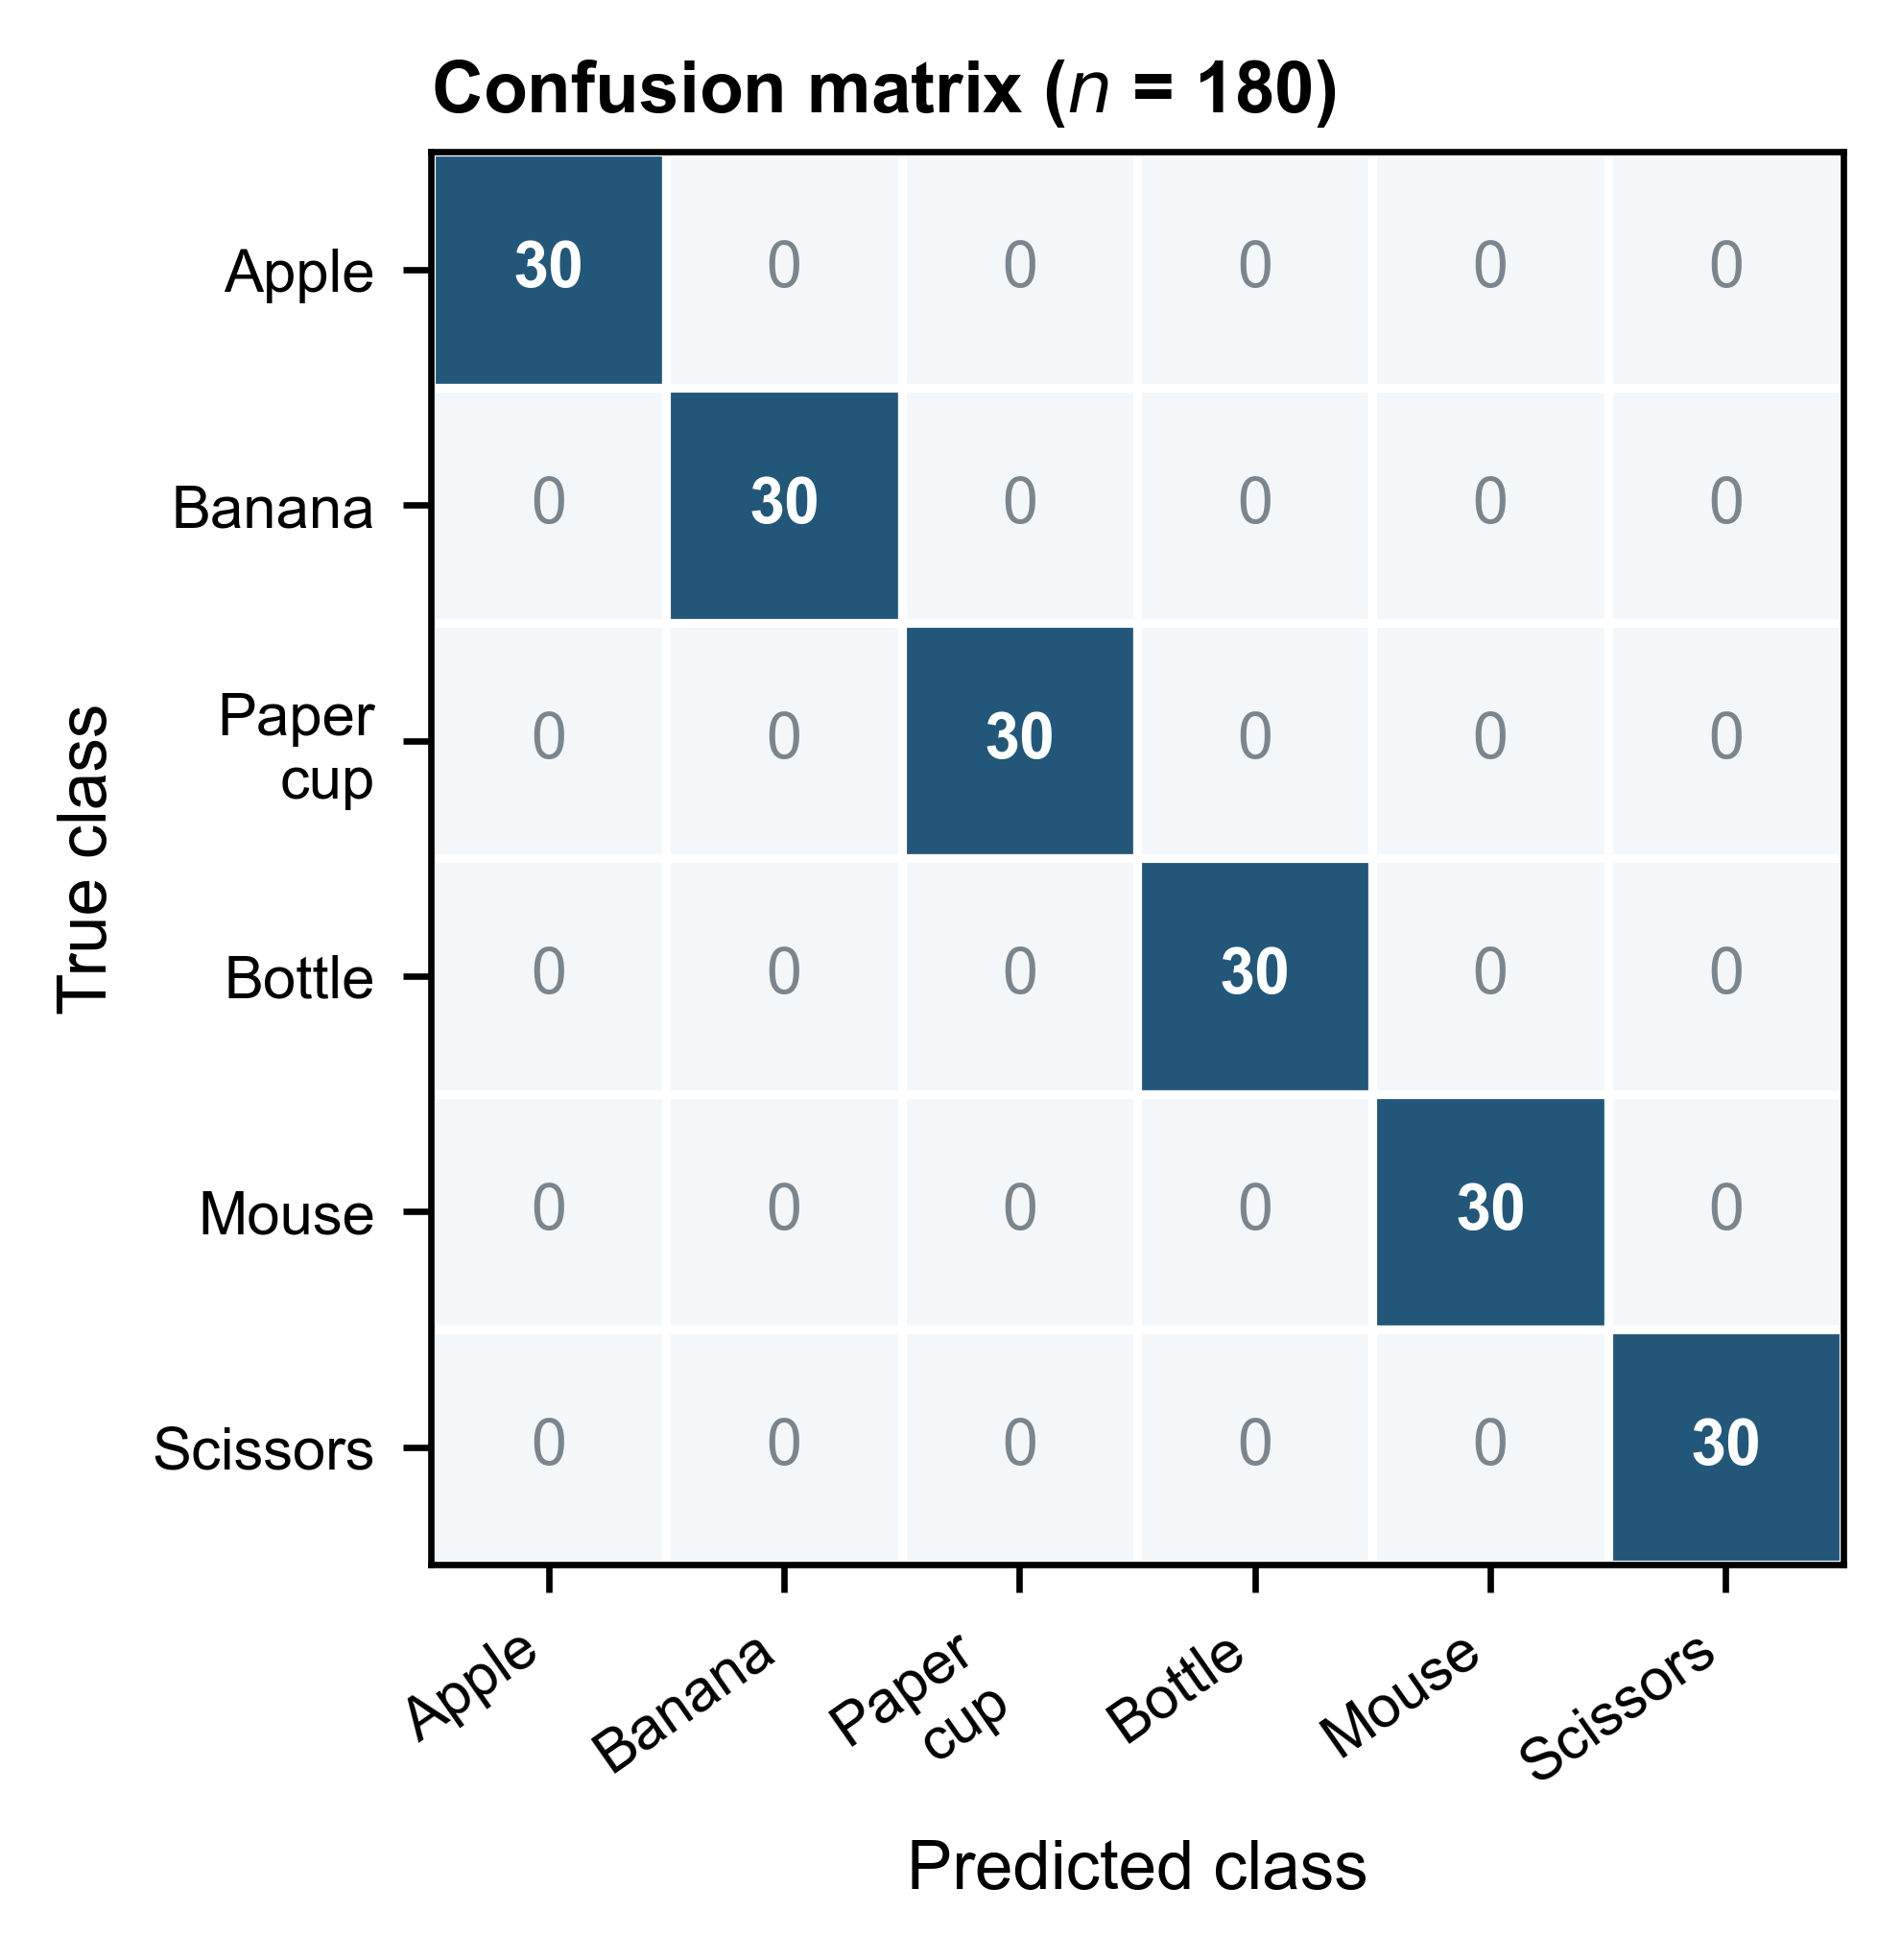
\includegraphics[width=0.72\textwidth]{figS1.png}
\par
\begin{flushleft}
\small
\textbf{Figure S1.} Confusion matrix for the separate closed-set controlled visual test (180 images; 30 images per class). All observations lie on the diagonal under the fixed viewpoint, background, and lighting conditions.
\end{flushleft}
\end{figure}
\end{document}
